\documentclass[10pt,a4paper,twocolumn]{article}
\usepackage[utf8]{inputenc}
\usepackage[francais]{babel}
\usepackage[T1]{fontenc}
\usepackage{amsmath}
\usepackage{amsfonts}
\usepackage{amssymb}
\usepackage{graphicx}
\title{Tiny Internet Project}
\author{Guillaume \textsc{Huysmans}, Martin \textsc{Lempereur}}
\begin{document}
\maketitle

\section{Introduction}
Le but de ce projet était de reconstruire une certaine topologie (voir figure \ref{fig:topo}) composée de différents AS eux-mêmes constitués de différents routeurs, à l'instar d'Internet. En plus de cela, nous devions paramétrer BGP sur ces routeurs. Enfin, nous devions configurer les filtres BGP pour que l'émission des routes respecte les différents liens commerciaux décrits dans l'énoncé.
\begin{figure}[h]
	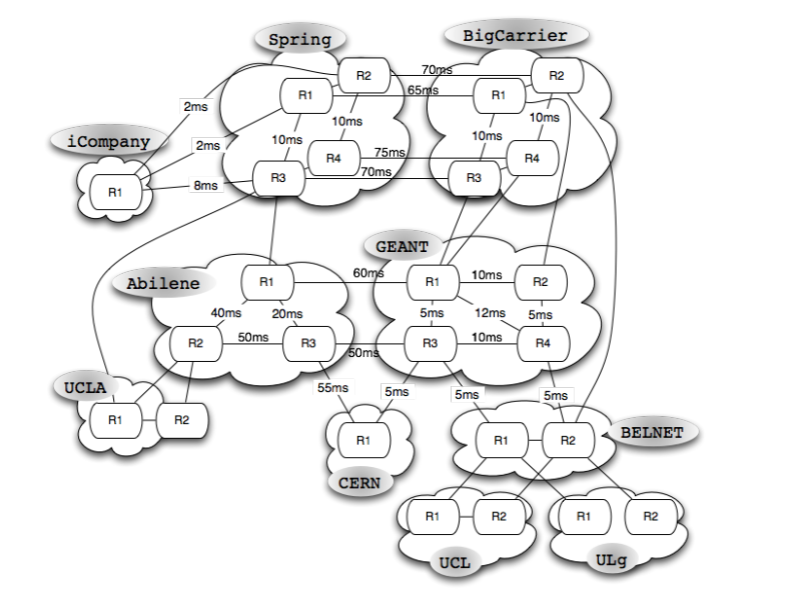
\includegraphics[width=\columnwidth]{topo.png}
	\caption{Topologie de l'énoncé}
	\label{fig:topo}
\end{figure}

\section{Création de la topologie}
En premier lieu, nous avons créé l'ensemble des nœuds présents sur la topologie. Ensuite, nous avons associé au nom de chaque AS son numéro et à chaque nœud, cet ASN.
Après cela, il nous restait à créer les liens. Pour cela, nous avons déterminé deux types de liens :
\begin{enumerate}
	\item les liens internes, présents au sein d'un même AS, permettent à l'aide d'IGP à un routeur de connaître tous les autres de cet AS.
	\item les liens externes connectent les routeurs de bordure entre eux et permettent l'échange de routes BGP.
\end{enumerate}

\section{Configuration des routeurs BGP}
Pour chaque routeur BGP (donc en bordure d'AS), on lui dit quel réseau il gère et quels sont ses voisins avec lesquels il devra échanger des messages en n'oubliant pas d'autoriser les connexions.

\section{Filtres de routage}
Nous avons déterminé les différents liens commerciaux qui existaient entre chaque AS. Une fois cela fait, il ne restait plus plus qu'à ajouter les filtres afin de respecter le tableau \ref{tab:rels}.
\begin{table}[h]
	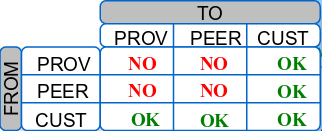
\includegraphics[width=\columnwidth]{comlink.png}
	\caption{Relations interdomaines (source : cours de \textit{Réseaux II}, Bruno \textsc{Quoitin})}
	\label{tab:rels}
\end{table}

\section{Problèmes rencontrés}
Un souci que nous n'avons pas pu corriger est que les routeurs de bordure n'arrivent pas à communiquer les routes BGP calculées à d'autres routeurs que ceux qui ont un lien direct avec eux au sein de leur AS.
Par exemple, R3 de Spring ne peut communiquer les routes BGP à R2 alors que R1 et R4, eux, les connaissent (et pourtant, il existe une route IGP de R3 vers R2).

\section{Outils utilisés}
Pour nous simplifier l'écriture de notre script et éviter de nombreuses erreurs (par copier-coller), nous avons utilisé \texttt{m4}, un puissant outil de remplacement de texte.
Ainsi, nous avons pu, à plusieurs reprises, regrouper quelques commandes en une seule \textit{macro} et rendre le script bien plus lisible. Ces macros sont définies dans \texttt{shortcuts.m4}, voici les principales :
\begin{itemize}
\item \texttt{NODE} : créer un nœud avec une adresse IP (<<~déduite~>> à partir du nom de l'AS)
	\begin{itemize}
		\item Nom d'AS
		\item Numéro du routeur dans l'AS
		\item Sous-réseau
	\end{itemize}
\item \texttt{LINK} : créer un lien bidirectionnel entre deux routeurs BGP (iBGP ou eBGP)
	\begin{itemize}
		\item Nom du premier AS
		\item Numéro du routeur dans le premier AS
		\item Nom du second AS
		\item Numéro du routeur dans le second AS
		\item Coût du lien
	\end{itemize}
\item \texttt{ILINK} : comme \texttt{LINK} mais au sein d'un seul AS (et donc configurer un lien IGP en plus)
\item \texttt{PROVIDER} : déclarer un fournisseur auquel on ne transmettra pas les routes d'autres fournisseurs ou de pairs (afin d'éviter de payer à sa place).
\item \texttt{PEER} : déclarer un pair auquel on ne transmettra pas les routes d'autres fournisseurs et pairs (pour la même raison que ci-dessus).
\end{itemize}

\end{document}
